\chapter{Reinforcement learning}
\label{chap:reinforcement}

So far, all the learning problems we have looked at have been either
{\em unsupervised}, in that we are given data and no expected outputs,
or {\em supervised}, that is, for each training input $\ex{x}{i}$, we
are told which value $\ex{y}{i}$ should be the output.  A very
different problem setting is {\em reinforcement learning}\index{reinforcement learning}, in which
the learning system is not directly told which outputs go with which
inputs.  Instead, there is an interaction of the form:
\begin{compactitem}
\item Learner observes {\em input} $\ex{s}{i}$
\item Learner generates {\em output} $\ex{a}{i}$
\item Learner observes {\em reward} $\ex{r}{i}$
\item Learner observes {\em input} $\ex{s}{i+1}$
\item Learner generates {\em output} $\ex{a}{i+1}$
\item Learner observes {\em reward} $\ex{r}{i+1}$
\item $\ldots$
\end{compactitem}
The learner is supposed to find a {\em policy}\index{reinforcement learning!policy}\index{policy!reinforcement learning}, mapping $s$ to $a$,
that maximizes expected reward over time.

\begin{center}
  \begin{tikzpicture}[main node/.style={draw,rounded corners,font=\Large},
                      arr/.style={->, thick, shorten <=5pt, shorten >=5pt,}]
    \node[main node] (rl) at (0,1) {Learner};
    \node[main node] (env) at (0,-1) {Environment};
    \draw (env.west) edge[arr, bend left=50, looseness=1.1]
      node[right] {reward} ($(rl.west) + (0, -0.1)$);
    \draw ($(env.west) + (0,-0.1)$) edge[arr, bend left=70, looseness=1.5]
      node[left] {state} ($(rl.west) + (0, 0.1)$);
    \draw (rl.east) edge[arr, bend left=70, looseness=1.5]
      node[right] {action} (env.east);
  \end{tikzpicture}
\end{center}

This problem setting is equivalent to an {\em online} supervised
learning under the following assumptions:
\begin{enumerate}
\item The space of possible outputs is binary
(e.g., $\{+1, -1\}$) and the space of possible rewards is binary
(e.g., $\{+1, -1\}$); 
\item $\ex{s}{i}$ is independent of all previous $\ex{s}{j}$ and
  $\ex{a}{j}$; and
\item $\ex{r}{i}$ depends only on $\ex{s}{i}$ and $\ex{a}{i}$.  
\end{enumerate}
In this
case, for any experience tuple $(\ex{s}{i}, \ex{a}{i}, \ex{r}{i})$, we
can generate a supervised training example, which is equal to
$(\ex{s}{i}, \ex{a}{i})$ if $\ex{r}{i} = +1$ and $(\ex{s}{i},
-\ex{a}{i})$ otherwise.
\question{What supervised-learning loss function would this objective
  correspond to?}

Markov decision processes form the basis for reinforcement learning,
and as such, we began in Section~\ref{sec:finding_mdp_policies} with a
discussion of how to find optimal policies for {\sc mdp}s when the
{\sc mdp} is completely known in advance.  However, in many
scenarios, full information about the
{\sc mdp} is unavailable.  For example, consider the case when the above
three assumptions do not hold.  When we relax assumption 1 above, we
have the class of {\em bandit problems}\index{bandit problem}, which we discuss in
Section~\ref{bandit}.  If we relax assumption 2, but assume that the
environment that the agent is interacting with is an {\sc mdp}, so
that $\ex{s}{i}$ depends only on $\ex{s}{i-1}$ and $\ex{a}{i-1}$ then
we are in the classical {\em reinforcement-learning} setting, which we
discuss in Section~\ref{rl}.  Weakening the assumptions further, for
instance, not allowing the learner to observe the current state
completely and correctly, makes the problem into a {\em partially
  observed MDP}\index{Markov decision policy!partially observed MDP} ({\sc pomdp}), which is substantially more difficult,
and beyond the scope of this class.


%%%%%%%%%%%%%%%%%%%%%%%%%%%%%%%%%%%%%%%%%%%%%%%%%%%%%%%%%%%%%%%%%%%%%%%%%%%%%
\section{Bandit problems}
\label{bandit}

A basic bandit problem is given by
\begin{itemize}
\item A set of actions $\mathcal A$;
\item A set of reward values $\mathcal R$; and
% \item A probabilistic reward function $R: A \rightarrow \text{Dist}(\R)$ where
%   $R(a)$ is drawn from a probability distribution over possible 
%   reward values in $\mathcal R$ conditioned on which action is
%   selected.  Each time the agent takes an action, a new value is drawn
%   from this distribution.
\item A probabilistic reward function $R: {\mathcal A} \times {\mathcal R} \rightarrow \mathbb{R}$, i.e. 
  $R$ is a function that takes an action and a reward and returns the probability of getting that reward conditioned on that action being taken, 
  $R(a, r) = p({\rm reward} = r \, |\, {\rm action} = a)$.
  This is analogous to how the transition function $T$ is defined.
  Each time the agent takes an action, a new value is drawn
  from this distribution.
\end{itemize}

The most typical bandit problem has $\mathcal R = \{0, 1\}$ and
$\lvert \mathcal A \rvert = k$. 
This is called a {\em $k$-armed bandit problem}\index{bandit problem!k-armed bandit}.
\note{Why?  Because in English slang, ``one-armed bandit'' is a name
  for a slot machine (an old-style gambling machine where you put a
  coin into a slot and then pull its arm to see if you get a payoff.)
  because it has one arm and takes your money!
  What we have here is a similar sort of machine, but with $k$ arms.}
There is a lot of mathematical literature on optimal strategies for
$k$-armed bandit problems under various assumptions.  The important
question is usually one of {\em exploration versus exploitation}\index{reinforcement learning!exploration vs. exploitation}.
Imagine that you have tried each action 10 times, and now you have
estimates $\hat{R}(a_j, r)$ for the probabilities $R(a_j, r)$ for reward $r$ given action $a_j$.  Which arm
should you pick next?  You could
\begin{description}
\item{\bf exploit} your knowledge, and choose the arm with the highest
  value of $\hat{R}(a_j, r)$ on all future trials; or 
\item{\bf explore} further, by trying some or all actions more times,
  hoping to get better estimates of the $R(a_j, r)$ values.
\end{description}
The theory ultimately tells us that, the longer our horizon $H$ (or,
similarly, closer to $1$ our discount factor), the more time we should
spend exploring, so that we don't converge prematurely on a bad choice
of action.
\question{Why is it that ``bad'' luck during exploration is more
  dangerous than ``good'' luck?  Imagine that there is an action that
  generates reward value 1 with probability 0.9, but the first three
  times you try it, it generates value 0.  How might that cause difficulty?  Why
  is this more dangerous than the situation when an action that
  generates reward value 1 with probability 0.1 actually generates
  reward 1 on the first three tries?
}
\note{There is a setting of supervised learning, called {\em active
    learning}\index{active learning}, where instead of being given a training set, the
  learner gets to select values of $x$ and the environment gives back
  a label $y$;  the problem of picking good $x$ values to query is
  interesting, but the problem of deriving a hypothesis from $(x, y)$
  pairs is the same as the supervised problem we have been studying.}
Note that what makes this a very different kind of problem from the
batch supervised learning setting is that:
\begin{itemize}
\item The agent gets to influence what data it gets (selecting $a_j$
  gives it another sample from $R(a_j, r)$), and
\item The agent is penalized for mistakes it makes while it is
  learning (if it is trying to maximize the expected reward $\sum_r r
  \cdot R(a_j, r)$ it
  gets while behaving).
\end{itemize}

In a {\em contextual} bandit problem\index{bandit problem!contextual bandit problem}, you have multiple possible
states, drawn from some set $\mathcal S$, and a separate bandit
problem associated with each one.

Bandit problems are an essential sub-component of reinforcement
learning.  It's important to be aware of the issues, but we will not
study solutions to them in this class.

\section{Sequential problems}
\label{rl}
In the more typical (and difficult!) case, we can think of our
learning agent interacting with an {\sc mdp}, where it knows $\mathcal
S$ and $\mathcal A$, but not $T(s,a,s')$ or $R(s,a)$.  The learner can
interact with the environment by selecting actions.  So, this is
somewhat like a contextual bandit problem, but more complicated,
because selecting an action influences not only what the immediate
reward will be, but also what state the system ends up in at the next
time step and, therefore, what additional rewards might be available
in the future.  Note that for simplicity, in the following we use the
deterministic reward function $R(s,a)$ defined in the last chapter,
rather than the probabilistic one defined above for the bandit problem.

A {\em reinforcement-learning ({\sc rl}) algorithm}\index{reinforcement learning!RL algorithm} is a kind of a policy that
depends on the whole history of states, actions, and rewards and
selects the next action to take.  There are several different ways to
measure the quality of an {\sc rl} algorithm, including:
\begin{itemize}
  \item Ignoring the $r_t$ values that it gets {\em while} learning,
    but consider how many interactions with the environment are
    required for it to learn a policy $\pi: \mathcal{S} \rightarrow 
    \mathcal{A}$ that is nearly optimal.
  \item Maximizing the expected discounted sum of total rewards while
    it is learning.
\end{itemize}
Most of the focus is on the first criterion, because the second one is
very difficult.  The first criterion is reasonable when the
learning can take place somewhere safe (imagine a robot learning,
inside the robot factory, where it can't hurt itself too badly) or in
a simulated environment.

Approaches to reinforcement-learning differ significantly according to
what kind of hypothesis or model they learn.  In the following
sections, we consider two simple approaches: model-based learning
(Section~\ref{sec:rl_model_based}) and policy search
(Section~\ref{sec:rl_policy_search}).  An important
approach, Q-learning, is presented in Section~\ref{sec:q_learning}.

%%%%%%%%%%%%%%%%%%%%
\subsection{Model-based RL}
\label{sec:rl_model_based}

The conceptually simplest approach to {\sc rl} is to model $R$ and
$T$ from the data we have gotten so far, and then use those models,
together with an algorithm for solving {\sc mdp}s (such as value
iteration) to find a policy that is near-optimal given the current
models.

Assume that we have had some set of interactions with the environment,
which can be characterized as a set of tuples of the form $(\ex{s}{t}, \ex{a}{t}, \ex{r}{t}, \ex{s}{t+1})$.

Because the transition function ${T}(s, a, s')$ specifies
probabilities, multiple observations of $(s, a, s')$ may be needed to
model the function.  One approach to this task of building a model
$\hat{T}(s, a, s')$ for the true ${T}(s,a,s')$ is to estimate it using
a simple counting strategy,
\begin{equation}
  \hat{T}(s,a,s') = \frac{\#(s,a,s') + 1}{\#(s,a) + \left|
      \mathcal{S}\right|}
\,.  
\end{equation}
Here, $\#(s, a, s')$ represents the
number of times in our data set we have the situation where
$s_t = s, a_t = a, s_{t+1} = s'$ and $\#(s, a)$ represents the number
of times in our data set we have the situation where
$s_t = s, a_t = a$.  \question{Prove to yourself that
  $\#(s,a) = \sum_{s'} \#(s,a,s')$.}

Adding 1 and $\left|\mathcal{S}\right|$ to the numerator and
denominator, respectively, are a form of smoothing called the {\em
  Laplace correction}\index{reinforcement learning!Laplace correction}. It ensures that we never estimate that a
probability is 0, and keeps us from dividing by 0.  As the amount of
data we gather increases, the influence of this correction fades away.

In contrast, the reward function ${R}(s, a)$\index{reward function} (as we have specified it
in this text) is a {\em deterministic} function, such that knowing the
reward $r$ for a given $(s, a)$ is sufficient to fully determine the
function at that point.  In other words, our model $\hat{R}$ can simply be
a record of observed rewards, such that $\hat{R}(s, a) = r = R(s,a)$.

A more general case is when the reward function is {\em
  non-deterministic}, such that the reward $R(s, a)$ may vary with
each query.  In this case, an estimation strategy similar to that
employed for the model $\hat{T}$ could be used for building the model
$\hat{R}$, e.g.:
\begin{equation}
     \hat{R}(s,a) = \frac{\sum r \mid s, a}{\#(s,a)} 
\end{equation}
where 
\begin{equation}
\sum r \mid s, a = \sum_{\{t \mid s_t = s, a_t = a\}}
  \ex{r}{t}\;\;.
\end{equation}
Such an estimate would just be the average of the observed rewards for each $s, a$ pair.  
However, this general case is outside the scope of what we cover here.

Given empirical models $\hat{T}$ and $\hat{R}$ for the transition and reward functions,  
we can now solve the {\sc mdp} $(\mathcal S, \mathcal A, \hat{T}, \hat{R})$ 
to find an optimal policy using value iteration, or use a
finite-depth expecti-max search to find an action to take for a
particular state.

This technique is effective for problems with small state and action
spaces, where it is not too hard to get enough experience to model
$T$ and $R$ well; but it is difficult to generalize this method to
handle continuous (or very large discrete) state spaces, and is a
topic of current research.

%%%%%%%%%%%%%%%%%%%%
\subsection{Policy search}
\label{sec:rl_policy_search}

A very different strategy is to search directly for a good policy,
without first (or ever!) estimating the transition and reward models.
The strategy here is to define a functional form $f(s;\theta) = a$ for
the policy, where $\theta$ represents the parameters we learn from
experience. We choose $f$ to be differentiable, and often let
$f(s;\theta) = P(a)$, a probability distribution over our possible
actions.

Now, we can train the policy parameters using gradient descent:
    \begin{itemize}
    \item When $\theta$ has relatively low dimension, we can compute a
      numeric estimate of the gradient by running the policy multiple
      times for $\theta \pm \epsilon$, and computing the resulting
      rewards.
      \item When $\theta$ has higher dimensions (e.g., it is a
        complicated neural network), there are more clever algorithms,
        e.g., one called {\sc reinforce}, but they can often be
        difficult to get to work reliably.
    \end{itemize}

Policy search is a good choice when the policy has a simple known
form, but the model would be much more complicated to estimate.

%%%%%%%%%%%%%%%%%%%%
% \subsection{Value function learning}
% \label{sec:rl_value_function_learning}


%%%%%%%%%%%%%%%%%%%%%%%%%%%%%%%%%%%%%%%%%%%%%%%%%%%%%%%%%%%%%%%%%%%%%%%%%%%%%

% \begin{noticebox}
%   The following material on Q-learning
%   (Section~\ref{sec:q_learning}) is for your own elucidation.  It is
%   not being covered in the Fall 2021 semester of 6.036, and will not
%   be included in the final exam.
% \end{noticebox}

\subsection{Q-learning}

\label{sec:q_learning}

The most frequently used class of reinforcement learning algorithms learns neither explicit
transition and reward models nor a direct policy, but instead
concentrates on learning a value function.  It is a topic of current
research to describe exactly under what circumstances
value-function-based approaches are best, and there are a growing
number of methods that combine value functions, transition and reward
models and policies into a complex learning algorithm in an attempt to
combine the strengths of each approach.

% We will study two variations on value-function learning, both of which
% estimate the $Q$ function.
%
Specifically, we look at a variation on value-function learning which
estimates the $Q$ function.  This {\em Q-learning} algorithm\index{Q-learning algorithm} is the
most typical way of performing reinforcement learning.  Recall the
value-iteration update:\note{The thing that most students seem to get
  confused about is when we do value iteration and when we do Q
  learning.  Value iteration assumes you know $T$ and $R$ and just
  need to {\em compute} $Q$.  In $Q$ learning, we don't know or even
  directly estimate $T$ and $R$: we estimate $Q$ directly from
  experience!}
\begin{equation}
 Q(s,a) = R(s,a) + \gamma \sum_{s'} T(s,a,s')\max_{a'}Q(s',a')
\end{equation}
We will adapt this update to the {\sc rl} scenario, where we do not
know the transition function $T$ or reward function $R$.
\begin{codebox}
  \Procname{$\proc{Q-Learning}(\mathcal S, \mathcal A, s_0, \gamma,
                               \alpha)$}
  \li \For $s \in \mathcal{S}, a \in \mathcal{A}:$
  \li   \Do
          $Q[s, a] = 0$
        \End
  \li $s \gets s_0$ \Comment Or draw an $s$ randomly from $\mathcal S$
  \li \While True:
  \li   \Do
          $a \gets \text{select}\_\text{action}(s, Q)$
  \li     $r,s' \gets \text{execute}(a)$
  \li     $Q[s, a] = (1-\alpha)Q[s, a]
          + \alpha(r + \gamma \max_{a'}Q[s',a'])$
  \li     $s \gets s'$
\end{codebox}
Here, $\alpha$ represents the ``learning rate,'' which needs to decay
for convergence purposes, but in practice is often set to a
constant. 

Note that the update can be rewritten as
\begin{equation}
Q[s, a] \gets Q[s, a]
    - \alpha\left(Q[s,a] - (r + \gamma \max_{a'}
    Q[s',a'])\right)\,,
\end{equation}
which looks something like a gradient update!  
\note{It is actually not a gradient update, but later, when we
  consider function approximation, we will treat it as if it were.}
This is often called {\em temporal difference} learning method\index{reinforcement learning!temporal difference method},
because we make an update based on the difference between the
current estimated value of taking action $a$ in state $s$, which is
$Q[s, a]$, and the ``one-step'' sampled value of taking $a$ in $s$,
which is $r + \gamma \max_{a'}  Q[s',a']$.

You can see this method as a combination of two different iterative
processes that we have already seen:  the combination of an old
estimate with a new sample using a running average with a learning
rate $\alpha$, and the dynamic-programming update of a $Q$ value from
value iteration.


Our algorithm above includes a procedure called {\it select\_action},
which, given the current state $s$,  has to decide which action to
take.  If the $Q$ value is estimated very accurately and the agent is
behaving in the world, then generally we would want to choose the
apparently optimal action $\argmax{a \in \mathcal A} Q(s,a)$.  But, during
learning, the $Q$ value estimates won't be very good and exploration
is important.  However, exploring completely at random is also usually
not the best strategy while learning, because it is good to focus your
attention on the parts  of the state space that are likely to be
visited when executing a good policy (not a stupid one).

A typical action-selection strategy is the $\epsilon$-greedy strategy:
        \begin{itemize}
          \item with probability $1-\epsilon$, choose
            $\argmax{a \in \mathcal A} Q(s,a)$
          \item with probability $\epsilon$, choose the action $a \in \mathcal A$
            uniformly at random
        \end{itemize}


Q-learning has the surprising property that it is {\em guaranteed}
to converge to the actual optimal $Q$ function under fairly weak
conditions!  Any exploration strategy is okay as long as it tries every action
        infinitely often on an infinite run (so that it doesn't
        converge prematurely to a bad action choice).

Q-learning can be very sample-inefficient:  imagine a robot that has a
choice between moving to the left and getting a reward  of 1, then
returning to its initial state, or moving to the right and walking
down a 10-step hallway in order to get a reward of 1000, then returning
to its initial state.

\begin{center}
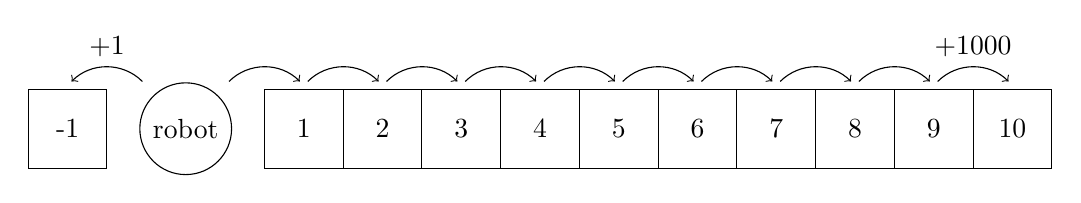
\begin{tikzpicture}
  \draw (-3,0) grid (-2,1);
  \draw (0,0) grid (10,1);
  \node[circle, draw] (robot) at (-1,.5) {robot};
  % right arrows
  \foreach \x in {1,2,3,4,5,6,7,8,9,10} {
    \coordinate (a) at (\x - 1.45, 1.1);
    \coordinate (b) at (\x - .55, 1.1);
    \draw (a) edge[->, bend left=45] coordinate (mid) (b);
    \node at (\x - .5, .5) {\x};
  }
  \node[above] (reward) at (mid) {+1000};

  % left arrow
  \coordinate (a) at (-2.45, 1.1);
  \coordinate (b) at (-1.55, 1.1);
  \draw (b) edge[->, bend right=45] node[above] {+1} (a);
  \node at (-2.5, .5) {-1};
\end{tikzpicture}
\end{center}

The first time the robot moves to the right and goes down the hallway,
it will update the $Q$ value for the last state on the hallway to
have a high value, but it won't yet understand that moving to the
right was a good choice.  The next time it moves down the hallway it
updates the value of the state before the last one, and so on.  After
10 trips down the hallway, it now can see that it is better to move to
the right than to the left. 

\setcounter{MaxMatrixCols}{20}

More concretely, consider the vector of Q values
$Q(0:10, \text{ right})$, representing the Q values for moving right
at each of the positions $0, \ldots, 9$. Then, for $\alpha=1$ and
$\gamma = 0.9$, 
\begin{equation}
Q(i, \text{ right}) = R(i, \text{ right})
                        + 0.9 \cdot \max_a Q(i+1, a)
\end{equation}
Starting with Q values of 0,
\begin{equation}
Q^{(0)}(0:10, \text{ right}) =
\begin{bmatrix} 0 & 0 & 0 & 0 & 0 & 0 & 0 & 0 & 0 & 0 & 0\end{bmatrix}
\end{equation}
\note{We are violating our usual notational conventions here, and
  writing $\ex{Q}{i}$ to mean the Q value function that results after
  the robot runs all the way to the end of the hallway, when executing
  the policy that always moves to the right.}
Since the only nonzero reward from moving right is
$R(9, \text{ right}) = 1000$, after our robot makes it down the
hallway once, our new Q vector is
\begin{equation}
Q^{(1)}(0:10, \text{ right}) = 
\begin{bmatrix} 0 & 0 & 0 & 0 & 0 & 0 & 0 & 0 & 0 & 1000 & 0\end{bmatrix}
\end{equation}
After making its way down the hallway again,
$Q(8, \text{ right}) = 0 + 0.9 \cdot Q(9, \text{ right}) = 900$
updates:
\begin{equation}
 Q^{(2)}(0:10, \text{ right}) = 
\begin{bmatrix}
  0 & 0 & 0 & 0 & 0 & 0 & 0 & 0 & 900 & 1000 & 0
\end{bmatrix} 
\end{equation}
Similarly,
\begin{align}
Q^{(3)}(0:10, \text{ right}) &= 
\begin{bmatrix}
  0 & 0 & 0 & 0 & 0 & 0 & 0 & 810 & 900 & 1000 & 0
\end{bmatrix} \\
Q^{(4)}(0:10, \text{ right}) &= 
\begin{bmatrix}
  0 & 0 & 0 & 0 & 0 & 0 & 729 & 810 & 900 & 1000 & 0
\end{bmatrix} \\
                             &\vdotswithin{=} \\
Q^{(10)}(0:10,  \text{ right}) &=
\begin{bmatrix}
  387.4 & 420.5 & 478.3 & 531.4 & 590.5 & 656.1 & 729 & 810
         & 900 & 1000 & 0
\end{bmatrix},
\end{align}
and the robot finally sees the value of moving right from position 0.
\note{We can see how this interacts with
  the exploration/exploitation dilemma:  from the perspective of
  $s_0$, it will seem, for a long time, that getting the immediate
  reward of $1$ is a better idea, and it would be easy to converge on
  that as a strategy without exploring the long hallway sufficiently.}
\question{Determine the Q value functions that will result from
  updates due to the robot always executing the ``move left'' policy.}


\subsection{Function approximation: Deep Q learning}
In our Q-learning algorithm above, we essentially keep track of each
$Q$ value in a table, indexed by $s$ and $a$. What do we do if
$\mathcal{S}$ and/or $\mathcal{A}$ are large (or continuous)?

We can use a function approximator like a neural network to store Q
values. For example, we could design a neural network that takes in
inputs $s$ and $a$, and outputs $Q(s,a)$. We can treat this as a
regression problem, optimizing the squared Bellman error, with loss:
\begin{equation}
\left(Q(s,a) - (r + \gamma \max_{a'}Q(s',a'))\right)^2\;\;,
\end{equation}
where $Q(s, a)$ is now the output  of the neural network.

There are actually several different architectural choices for using a
neural network to approximate $Q$ values:
\begin{itemize}
\item One network for each action $a_j$, that takes $s$ as input and
  produces $Q(s,  a_j)$ as output;
\item One single network that takes $s$ as input and produces a vector
  $Q(s, \cdot)$, consisting of the $Q$ values for each action; or
\item One single network that takes $s, a$ concatenated into a vector
  (if $a$ is discrete,  we would probably use a one-hot encoding,
  unless it had some useful internal structure) and produces $Q(s, a)$
  as output.
\end{itemize}

\note{For
continuous action spaces, it is increasingly popular to use a class of
methods called {\em actor-critic} methods\index{reinforcement!actor-critic methods}, which combine policy and
value-function learning.  We won't get into them in detail here,
though.}

The first two choices are only suitable for discrete (and not too big)
action sets.  The last choice can be applied for continuous actions,
but then it is  difficult to find $\argmax{\mathcal A} Q(s, a)$.  

There are not many theoretical guarantees about Q-learning with
function approximation and, indeed,  it can sometimes be fairly
unstable (learning to perform well for a while, and then getting
suddenly worse, for example).  But it has also had some significant
successes. 

One form of instability that we do know how to guard against is {\em
  catastrophic forgetting.}  In standard supervised learning, we
expect that the training $x$ values were drawn independently from some
distribution. \note{And, in fact, we routinely shuffle their order in
  the data file, anyway.}  But when a learning agent, such as a robot,
is moving through an environment, the sequence of states it encounters
will be temporally correlated. \note{For example, it might spend 12
  hours in a dark environment and then 12 in a light one.}  This can
mean that while it is in the dark, the neural-network weight-updates
will make the $Q$ function ``forget'' the value function for when it's
light.

One way to handle this is to use $\emph{experience replay}$\index{experience replay}, where we
save our $(s,a,r,s')$ experiences in a {\it replay buffer}.
Whenever we take a step in the world, we add the $(s,a,r,s')$ to the
replay buffer and use it to do a Q-learning update.  Then we also
randomly select some number of tuples from the replay buffer, and do
Q-learning updates based on them, as well.  In general it may help to
keep a {\em sliding window}\index{sliding window} of just the 1000 most recent experiences
in the replay buffer.  (A larger buffer will be necessary for
situations when the optimal policy might visit a large part of the
state space, but we like to keep the buffer size small for memory
reasons and also so that we don't focus on parts of the state space
that are irrelevant for the optimal policy.)
The idea is that it will help you propagate reward values through your
state space more efficiently if you do these updates. You can see it
as doing something like value iteration, but using samples of
experience rather than a known model. 

\subsection{Fitted Q-learning}
An alternative strategy for learning the $Q$ function that is somewhat
more robust than the standard $Q$-learning algorithm is a method
called {\em fitted Q}.\index{fitted Q-learning}

\begin{codebox}
  \Procname{$\proc{Fitted-Q-Learning}(\mathcal A, s_0, \gamma, \alpha,
    \epsilon, m)$}
  \li $s \gets s_0$ \Comment Or draw an $s$ randomly from $\mathcal S$
  \li $\mathcal D = \{\;\}$
  \li initialize neural-network representation of $Q$
  \li \While True: \Do
  \li  $\mathcal D_\text{new}$ = experience from executing $\epsilon$-greedy policy based
  on $Q$ for $m$ steps
\li $\mathcal D = \mathcal D \cup \mathcal D_\text{new}$ represented
as $(s, a, r, s')$ tuples
\li $D_\text{sup} = \{(\ex{x}{i}, \ex{y}{i})\}$  where $\ex{x}{i} =
(s, a)$ and $\ex{y}{i} = r + \gamma \max_{a' \in \mathcal A} Q(s',
a')$ 
  \li \;\;\;for each tuple $\ex{(s, a, r, s')}{i} \in \mathcal D$ 
  \li re-initialize neural-network representation of $Q$
  \li $Q = \text{supervised\_NN\_regression}(D_\text{sup})$
\End
\end{codebox}

Here, we alternate between using the policy induced  by the current
$Q$ function to gather a batch of data $\mathcal D_\text{new}$, adding
it to our overall data set $\mathcal D$, and then using supervised
neural-network training to learn a representation of the $Q$ value
function on the whole data set.  This method does not mix the
dynamic-programming phase (computing new $Q$ values based on old ones)
with the function approximation phase (training the neural network)
and avoids catastrophic forgetting.  The regression training in line 9
typically uses squared error as a loss function and would be trained
until the fit is good (possibly measured on held-out data).


% \section{Applications}
% \subsection{Atari games}
% \begin{itemize}
%   \item Input(s): 4 downsampled screen images (recent frames)
%   \item Output: discrete joystick command
%   \item Q-learning + experience replay + NN
%   \item Surprisingly effective, but
%     \begin{itemize}
%       \item not good at long-term planning ($\gamma = 0.99$)
%       \item not good when partially observable
%     \end{itemize}
% \end{itemize}
% \subsection{AlphaZero}
% Two player zero-sum complete information games can be solved using
% (a minor variant of) value iteration. It takes advantage of the fact
% that $V(s)$ for player 1 is basically $-V(s)$ for player 2.

% Q-learning works, too.
% \begin{description}
%   \item[1992:] TD-Gammon learns to play Backgammon at near expert
%     level. Uses hand-crafted board features $\phi(s)$ as input to
%     a neural network, trained with 1.5 million games of self play.
%   \item[2017:] Silver et al. use similar ideas at a much larger
%     scale in AlphaZero, and use a tree search to improve value
%     estimates and generate supervised training data.

%     AlphaZero learns to play Go, chess, and Shogi as well or better
%     than the best computer players.


% \end{description}


%%% Local Variables:
%%% mode: latex
%%% TeX-master: "top"
%%% End:
